%----------------------------------------------------------------------------------------
%	PACKAGES AND OTHER DOCUMENT CONFIGURATIONS
%----------------------------------------------------------------------------------------

\documentclass{article}
\renewcommand{\baselinestretch}{1.5} 
\usepackage[T1]{fontenc}
\usepackage{graphicx}

%%%%%%%%%%%%%%%%%%%%%%%%%%%%%%%%%%%%%%%%%
% Lachaise Assignment
% Structure Specification File
% Version 1.0 (26/6/2018)
%
% This template originates from:
% http://www.LaTeXTemplates.com
%
% Authors:
% Marion Lachaise & François Févotte
% Vel (vel@LaTeXTemplates.com)
%
% License:
% CC BY-NC-SA 3.0 (http://creativecommons.org/licenses/by-nc-sa/3.0/)
% 
%%%%%%%%%%%%%%%%%%%%%%%%%%%%%%%%%%%%%%%%%

%----------------------------------------------------------------------------------------
%	PACKAGES AND OTHER DOCUMENT CONFIGURATIONS
%----------------------------------------------------------------------------------------

\usepackage{amsmath,amsfonts,stmaryrd,amssymb} % Math packages

\usepackage{enumerate} % Custom item numbers for enumerations

\usepackage[ruled]{algorithm2e} % Algorithms

\usepackage[framemethod=tikz]{mdframed} % Allows defining custom boxed/framed environments

\usepackage{listings} % File listings, with syntax highlighting
\lstset{
	basicstyle=\ttfamily, % Typeset listings in monospace font
}

%----------------------------------------------------------------------------------------
%	DOCUMENT MARGINS
%----------------------------------------------------------------------------------------

\usepackage{geometry} % Required for adjusting page dimensions and margins

\geometry{
	paper=a4paper, % Paper size, change to letterpaper for US letter size
	top=2.5cm, % Top margin
	bottom=3cm, % Bottom margin
	left=2.5cm, % Left margin
	right=2.5cm, % Right margin
	headheight=14pt, % Header height
	footskip=1.5cm, % Space from the bottom margin to the baseline of the footer
	headsep=1.2cm, % Space from the top margin to the baseline of the header
	%showframe, % Uncomment to show how the type block is set on the page
}

%----------------------------------------------------------------------------------------
%	FONTS
%----------------------------------------------------------------------------------------

\usepackage[utf8]{inputenc} % Required for inputting international characters
\usepackage[T1]{fontenc} % Output font encoding for international characters

\usepackage{XCharter} % Use the XCharter fonts

%----------------------------------------------------------------------------------------
%	COMMAND LINE ENVIRONMENT
%----------------------------------------------------------------------------------------

% Usage:
% \begin{commandline}
%	\begin{verbatim}
%		$ ls
%		
%		Applications	Desktop	...
%	\end{verbatim}
% \end{commandline}

\mdfdefinestyle{commandline}{
	leftmargin=10pt,
	rightmargin=10pt,
	innerleftmargin=15pt,
	middlelinecolor=black!50!white,
	middlelinewidth=2pt,
	frametitlerule=false,
	backgroundcolor=black!5!white,
	frametitle={Command Line},
	frametitlefont={\normalfont\sffamily\color{white}\hspace{-1em}},
	frametitlebackgroundcolor=black!50!white,
	nobreak,
}

% Define a custom environment for command-line snapshots
\newenvironment{commandline}{
	\medskip
	\begin{mdframed}[style=commandline]
}{
	\end{mdframed}
	\medskip
}

%----------------------------------------------------------------------------------------
%	FILE CONTENTS ENVIRONMENT
%----------------------------------------------------------------------------------------

% Usage:
% \begin{file}[optional filename, defaults to "File"]
%	File contents, for example, with a listings environment
% \end{file}

\mdfdefinestyle{file}{
	innertopmargin=1.6\baselineskip,
	innerbottommargin=0.8\baselineskip,
	topline=false, bottomline=false,
	leftline=false, rightline=false,
	leftmargin=2cm,
	rightmargin=2cm,
	singleextra={%
		\draw[fill=black!10!white](P)++(0,-1.2em)rectangle(P-|O);
		\node[anchor=north west]
		at(P-|O){\ttfamily\mdfilename};
		%
		\def\l{3em}
		\draw(O-|P)++(-\l,0)--++(\l,\l)--(P)--(P-|O)--(O)--cycle;
		\draw(O-|P)++(-\l,0)--++(0,\l)--++(\l,0);
	},
	nobreak,
}

% Define a custom environment for file contents
\newenvironment{file}[1][File]{ % Set the default filename to "File"
	\medskip
	\newcommand{\mdfilename}{#1}
	\begin{mdframed}[style=file]
}{
	\end{mdframed}
	\medskip
}

%----------------------------------------------------------------------------------------
%	NUMBERED QUESTIONS ENVIRONMENT
%----------------------------------------------------------------------------------------

% Usage:
% \begin{question}[optional title]
%	Question contents
% \end{question}

\mdfdefinestyle{question}{
	innertopmargin=1.2\baselineskip,
	innerbottommargin=0.8\baselineskip,
	roundcorner=5pt,
	nobreak,
	singleextra={%
		\draw(P-|O)node[xshift=1em,anchor=west,fill=white,draw,rounded corners=5pt]{%
		Question \theQuestion\questionTitle};
	},
}

\newcounter{Question} % Stores the current question number that gets iterated with each new question

% Define a custom environment for numbered questions
\newenvironment{question}[1][\unskip]{
	\bigskip
	\stepcounter{Question}
	\newcommand{\questionTitle}{~#1}
	\begin{mdframed}[style=question]
}{
	\end{mdframed}
	\medskip
}

%----------------------------------------------------------------------------------------
%	WARNING TEXT ENVIRONMENT
%----------------------------------------------------------------------------------------

% Usage:
% \begin{warn}[optional title, defaults to "Warning:"]
%	Contents
% \end{warn}

\mdfdefinestyle{warning}{
	topline=false, bottomline=false,
	leftline=false, rightline=false,
	nobreak,
	singleextra={%
		\draw(P-|O)++(-0.5em,0)node(tmp1){};
		\draw(P-|O)++(0.5em,0)node(tmp2){};
		\fill[black,rotate around={45:(P-|O)}](tmp1)rectangle(tmp2);
		\node at(P-|O){\color{white}\scriptsize\bf !};
		\draw[very thick](P-|O)++(0,-1em)--(O);%--(O-|P);
	}
}

% Define a custom environment for warning text
\newenvironment{warn}[1][Warning:]{ % Set the default warning to "Warning:"
	\medskip
	\begin{mdframed}[style=warning]
		\noindent{\textbf{#1}}
}{
	\end{mdframed}
}

%----------------------------------------------------------------------------------------
%	INFORMATION ENVIRONMENT
%----------------------------------------------------------------------------------------

% Usage:
% \begin{info}[optional title, defaults to "Info:"]
% 	contents
% 	\end{info}

\mdfdefinestyle{info}{%
	topline=false, bottomline=false,
	leftline=false, rightline=false,
	nobreak,
	singleextra={%
		\fill[black](P-|O)circle[radius=0.4em];
		\node at(P-|O){\color{white}\scriptsize\bf i};
		\draw[very thick](P-|O)++(0,-0.8em)--(O);%--(O-|P);
	}
}

% Define a custom environment for information
\newenvironment{info}[1][Info:]{ % Set the default title to "Info:"
	\medskip
	\begin{mdframed}[style=info]
		\noindent{\textbf{#1}}
}{
	\end{mdframed}
}
 % Include the file specifying the document structure and custom commands

%----------------------------------------------------------------------------------------
%	ASSIGNMENT INFORMATION
%----------------------------------------------------------------------------------------

\title{Detection and Prevention of SQL Injection Attack} % Title of the assignment

\author{Ciprian-Mihai Ceausescu\\ \texttt{ciprian-mihai.ceausescu@my.fmi.unibuc.ro}} % Author name and email address

\date{University of Bucharest --- \today} % University, school and/or department name(s) and a date

%----------------------------------------------------------------------------------------

\begin{document}

\maketitle % Print the title

%----------------------------------------------------------------------------------------
%	Introduction
%----------------------------------------------------------------------------------------

\section*{Introduction}
\hspace{10mm}\textbf{SQL} (Structure Query Language) injection is one of threats to the applications, which are Web-based
application, Mobile application and also Desktop application, which are connected to the database in order to make work with necessary data. By implementing SQL injection, the attacker can gain full access to the application or database. After this step, the attacker can remove or change significant data irresponsibly.
\\ \hspace*{10mm}Applications that do not properly validate the user’s input make them vulnerable against SQL injection. SQL Injection Attacks (SQLIA) occurs when an attacker is able to insert a series of malicious SQL statements into a query through manipulating user input data for execution by the back-end database. Using this type of threats, applications could be hacked easily and steal the confidential data by the attacker.
\\ \hspace*{10mm}Nowadays, the Internet is becoming a wide-spread information infrastructure. The Utilization and fast progress of
the Internet infrastructure has motivated the increasing amount of data stored in a database lately. Increasing the
number of users and the heavy dependence on digital information is led to the importance of securing data or
information spatially if this information about commercial, corporate businesses, institutions, organizations,
numerous financial transactions, health information, personal information and other internet based services. Via
Internet all web applications can be accessed using any web browsers that run on any operating systems. Web
applications have become the interface that is widely used to retrieve or insert these data or information. The
web application with a database that stores important information is one of the targets of the SQLIA, since the
databases are absolutely accessible by attacker by injecting SQL queries that are retrieved by web application. As
user information is frequently kept in these databases, important information is lost and the security violate.

%----------------------------------------------------------------------------------------
%	SQL Injection attack
%----------------------------------------------------------------------------------------

\section*{SQL Injection attack} 
\hspace*{10mm}SQL Injection is one of the most common threats to a database system in which the attacker adds SQL statement to an application form input box, to gain access the resources or make changes to data stored into database. Lack of input validation in applications causes attacker to be successful. In an SQL Injection attack, the attacker injects a string input through the application, which changes or manipulates the SQL statement to the attacker's advantage. An SQL Injection attack can harm the database in various ways, such as unauthorized manipulation of the database, or retrieval of sensitive data. It can also be used to execute system level commands that may cause the system to deny service to the application. This issue is very risky because it can cause data loss or misuse of data by parties who are not authorized and as result the functionality and confidentiality are destroyed. Basically, the process of SQLIA is illustrated in the following figure:
\hspace*{10mm} \\
\begin{center}
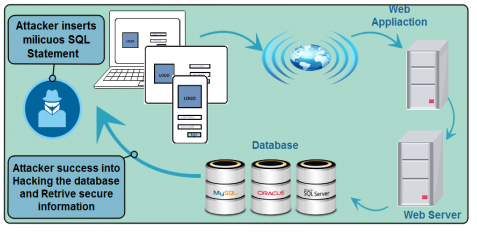
\includegraphics[scale=1]{1}
\end{center}

%----------------------------------------------------------------------------------------
%	Risks
%----------------------------------------------------------------------------------------

\section*{Risks} 
\hspace*{10mm}SQL injection is harmful and the risks associated with it provide motivation for attackers to attack the database. The main consequences of these vulnerabilities are attacks on the following characteristics:
\begin{enumerate}
\item \textbf{Authorization}: Critical data that are stored in a vulnerable SQL database may be altered by a successful
SQLIA.
\item \textbf{Authentication}: If there is no any proper control on input fields inside the authentication page, it may be
possible to login into a system as a normal user without knowing the authenticated user.
\item \textbf{Confidentially}: Usually databases are consisting of sensitive data such as personal information, credit card
numbers and / or social numbers. Therefore, loss of confidentially is a terrible problem with SQL Injection
vulnerability.
\item \textbf{Integrity}: By a successful SQLIA not only an attacker reads sensitive information, but also, it is possible to
change or delete this private information.
\item \textbf{Database Fingerprinting}: The attacker can determine the type of database being used in backend so that he
can use database-specific attacks that correspond to weakness in a particular database management system.
\end{enumerate}

%----------------------------------------------------------------------------------------
%	Classification of SQLIA
%----------------------------------------------------------------------------------------

\section*{Classical Types SQLIA}
\begin{enumerate}
\item \textbf{Tautologies} - Tautology-based attacks work through injecting code by one or more conditional SQL statement queries in order
to make the SQL command evaluate as a true condition such as (1=1) or (- -).
\begin{center}
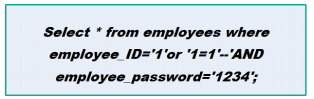
\includegraphics[scale=1]{2}
\end{center}
\item \textbf{Piggy-backed Query} - Piggy-backed queries is a type of attack that compromises a database using a query delimiter, such as
";", to inject additional query statements to the original query.
\begin{center}
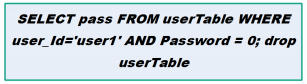
\includegraphics[scale=1]{3}
\end{center}
\item \textbf{Logically Incorrect} - Logically Incorrect attack takes advantage of the error messages that are returned by the
database for an incorrect query.
\begin{center}
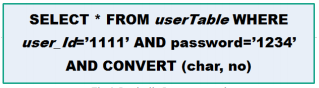
\includegraphics[scale=1]{4}
\end{center}
\item \textbf{Union query} - Union query injection is called as statement injection attack. In this attack, attacker insert
additional statement into the original SQL statement. 
\begin{center}
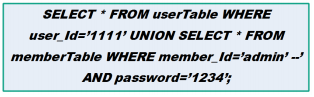
\includegraphics[scale=1]{5}
\end{center}
\item \textbf{Stored Procedure} - In this technique, attacker focuses on the stored procedures which are present in the database
system. Stored procedures run directly by the database engine. it is a piece of code which is exploitable. Stored
procedure gives true or false values for the authorized or unauthorized clients.
\begin{center}
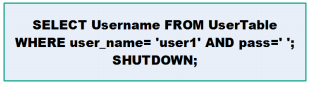
\includegraphics[scale=1]{6}
\end{center}
\item \textbf{Inference} - Using Inference attack enable the attacker changing the behavior of a database or application. This
type of attack can be classified into two well-known techniques, which are: Blind injection and timing attack.
\begin{center}
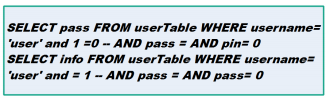
\includegraphics[scale=1]{7}
\end{center}
\begin{center}
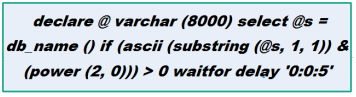
\includegraphics[scale=1]{8}
\end{center}
\item \textbf{Alternate Encodings} - This type of attack occurs when attacker modify the injection query via using alternate
encoding, such as hexadecimal, ASCII, and Unicode.
\begin{center}
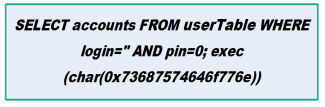
\includegraphics[scale=1]{9}
\end{center}
\end{enumerate}
%----------------------------------------------------------------------------------------
%	Project
%----------------------------------------------------------------------------------------
\section*{Project}
\begin{center}
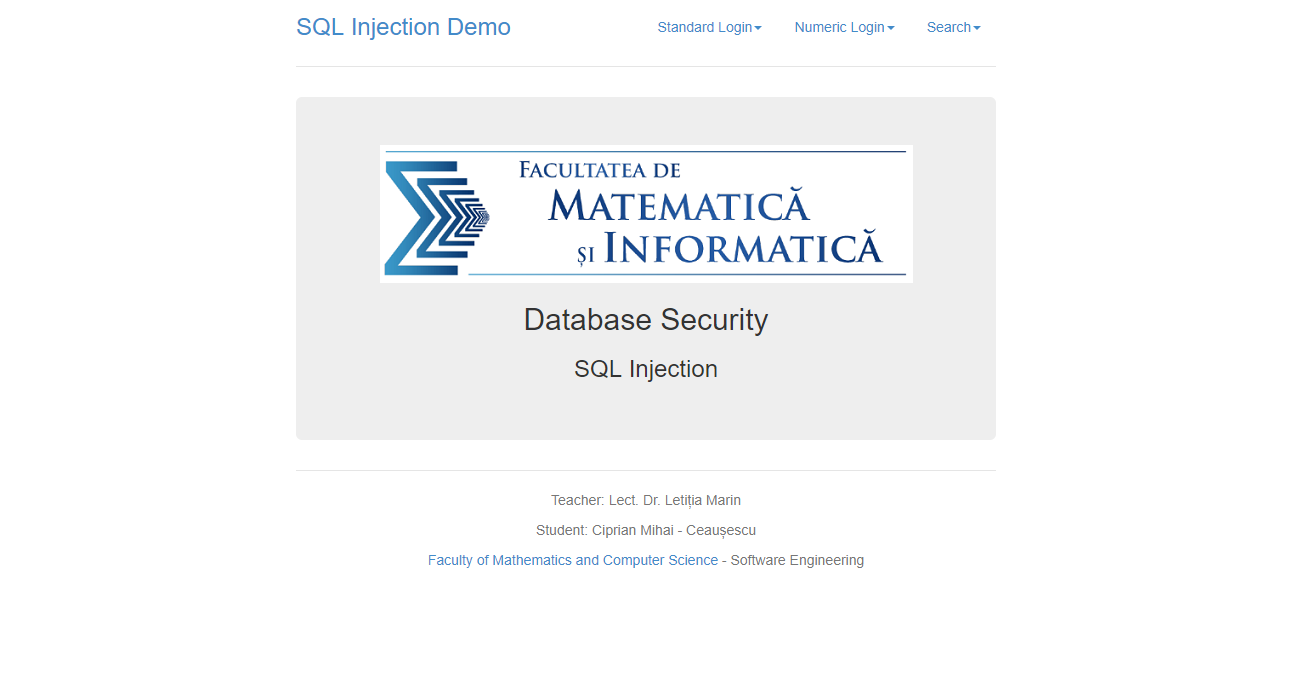
\includegraphics[scale=0.5]{f1}
\end{center}
\begin{center}
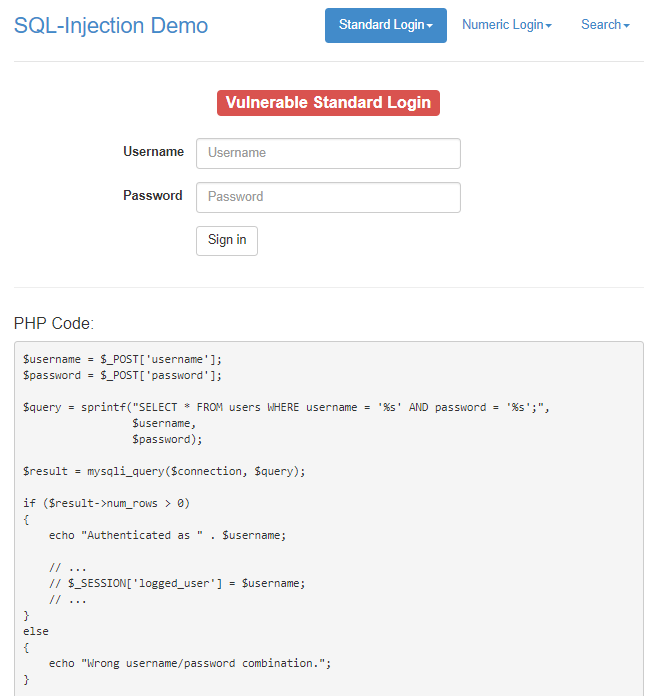
\includegraphics[scale=1]{f2}
\end{center}
\begin{center}
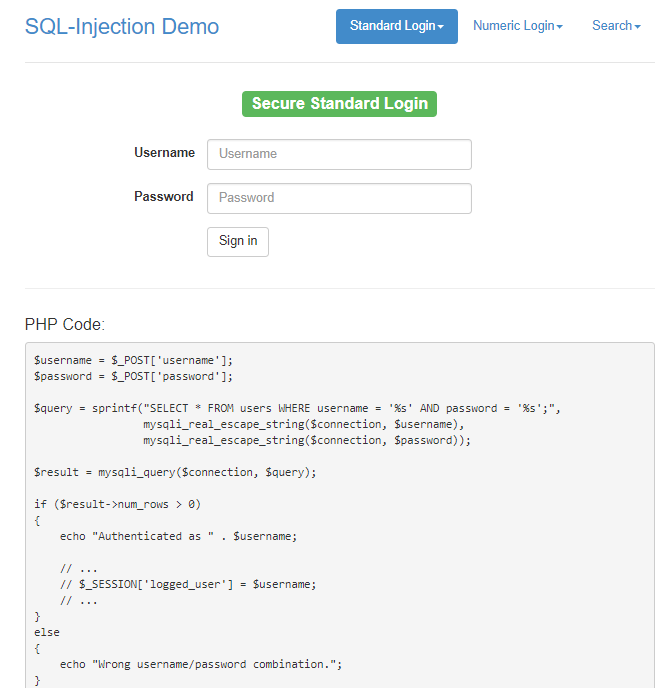
\includegraphics[scale=1]{f3}
\end{center}
\begin{center}
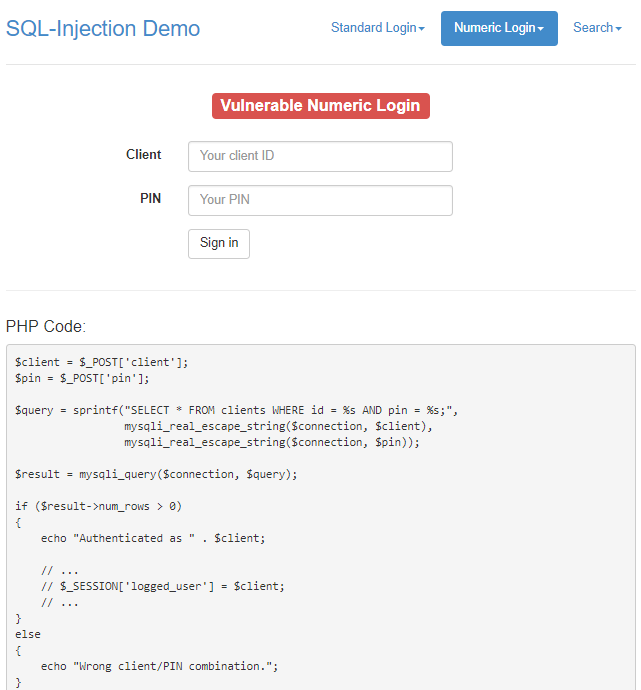
\includegraphics[scale=1]{f4}
\end{center}
\begin{center}
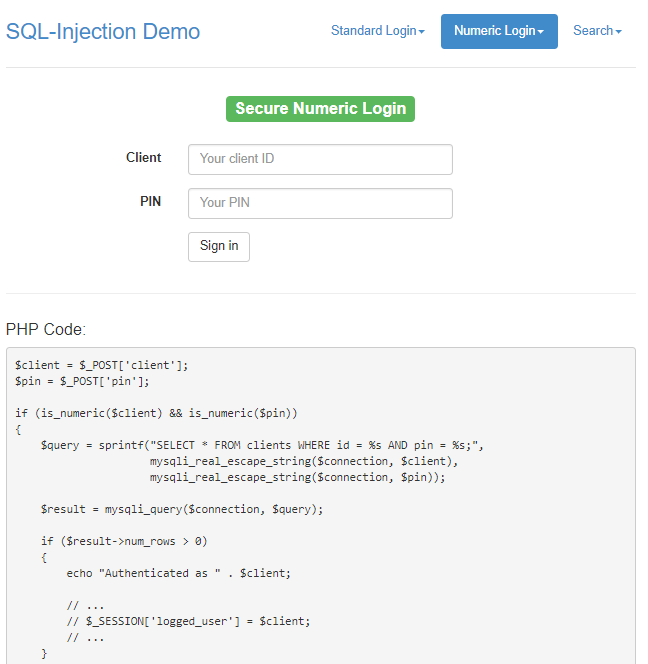
\includegraphics[scale=1]{f5}
\end{center}
\begin{center}
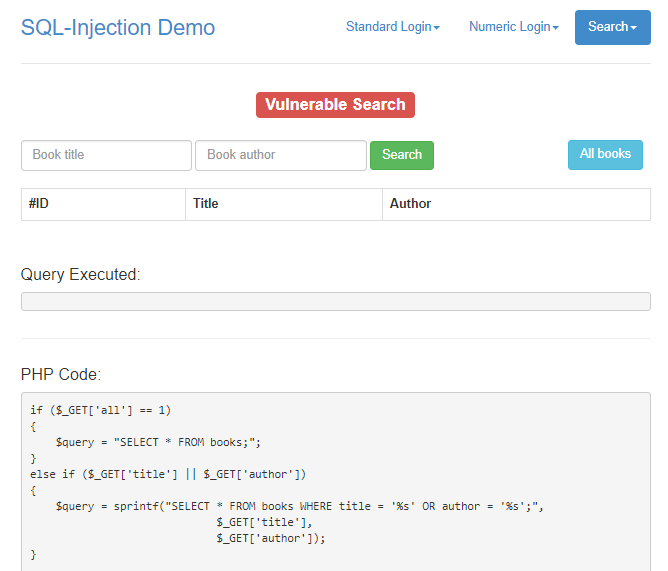
\includegraphics[scale=1]{f6}
\end{center}
\begin{center}
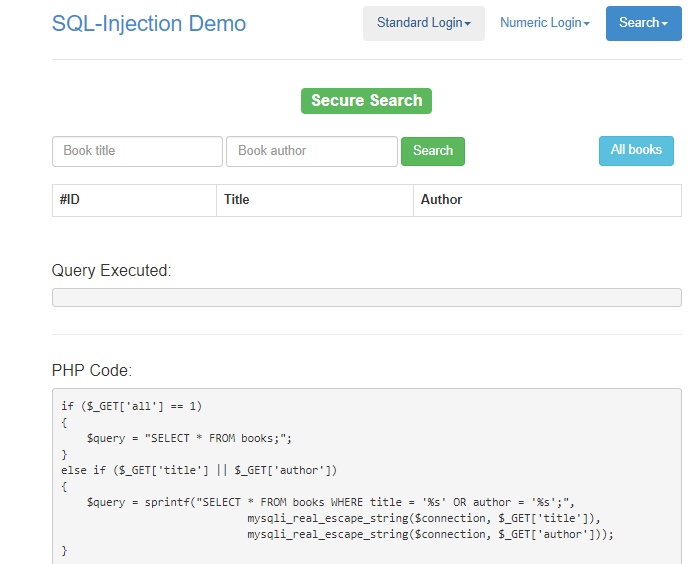
\includegraphics[scale=1]{f7}
\end{center}
%----------------------------------------------------------------------------------------
%	Bibliography
%----------------------------------------------------------------------------------------
\section*{Bibliography} 
\begin{itemize}
	\item \textbf{Detection and Prevention of SQL Injection Attack: A Survey}, Zainab S. Alwan and Manal F. Younis2
\end{itemize}
\end{document}
